\documentclass{beamer}
\usepackage[utf8]{inputenc}
\usepackage[czech]{babel}

\usetheme{Frankfurt}

\title{Virtuální sdílená tabule}
\author{Adam Šárek (SAR0083)}

\begin{document}
\begin{frame}
    \titlepage
\end{frame}

\begin{frame}{Obsah}
    \tableofcontents
\end{frame}



\section{Motivace}
\begin{frame}
    \frametitle{Motivace}
    \begin{itemize}
        \item Moderní webová aplikace
        \item Současná práce více uživatelů
        \item Podpora dotykových zařízení
        \item Implementace tmavého motivu
    \end{itemize}
\end{frame}



\section{Analýza stávajících řešení}
\subsection{Analýza stávajících řešení -- classroomscreen.com}
\begin{frame}
    \frametitle{Analýza stávajících řešení -- classroomscreen.com}
    \begin{figure}
        \centering
        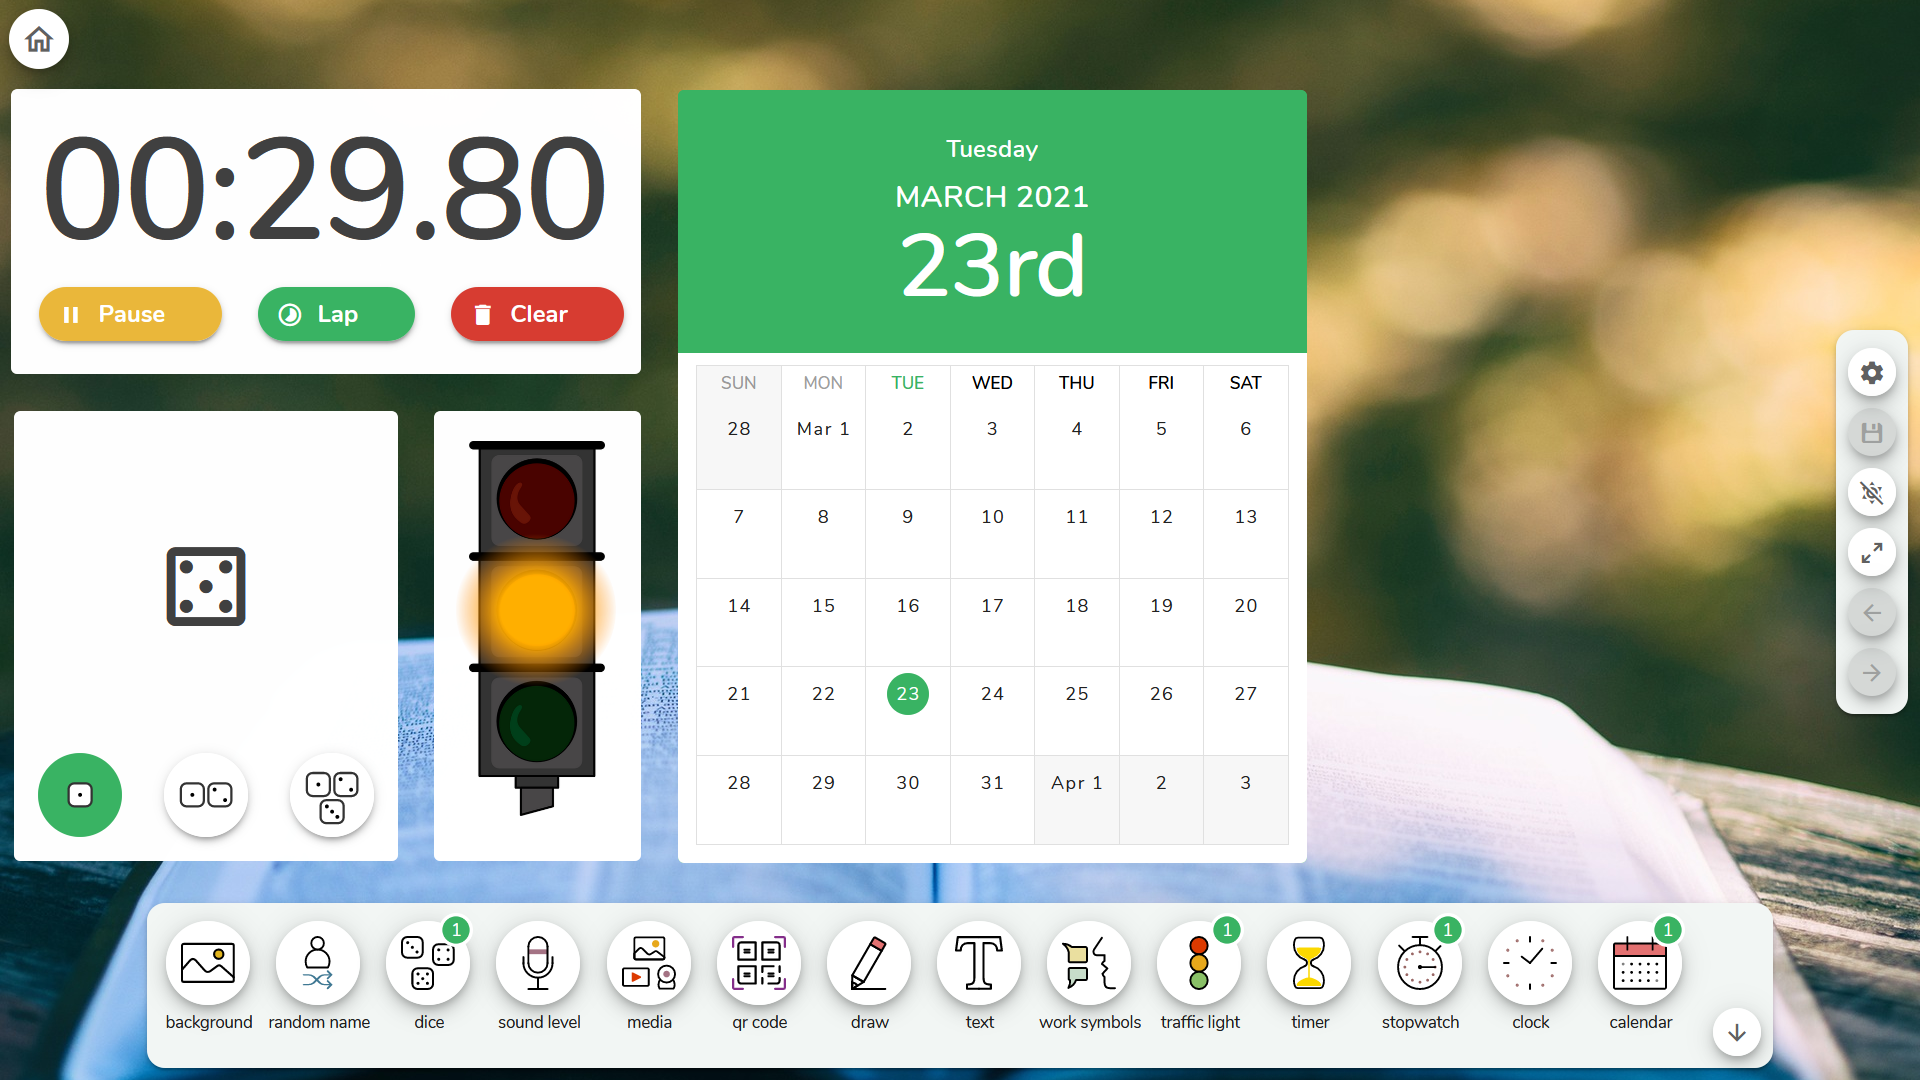
\includegraphics[width=1\textwidth]{Figures/classroomscreen.png}
        \caption{Snímek webu classroomscreen.com}
    \end{figure}
\end{frame}

\subsection{Analýza stávajících řešení -- whiteboard.fi}
\begin{frame}
    \frametitle{Analýza stávajících řešení -- whiteboard.fi}
    \begin{figure}
        \centering
        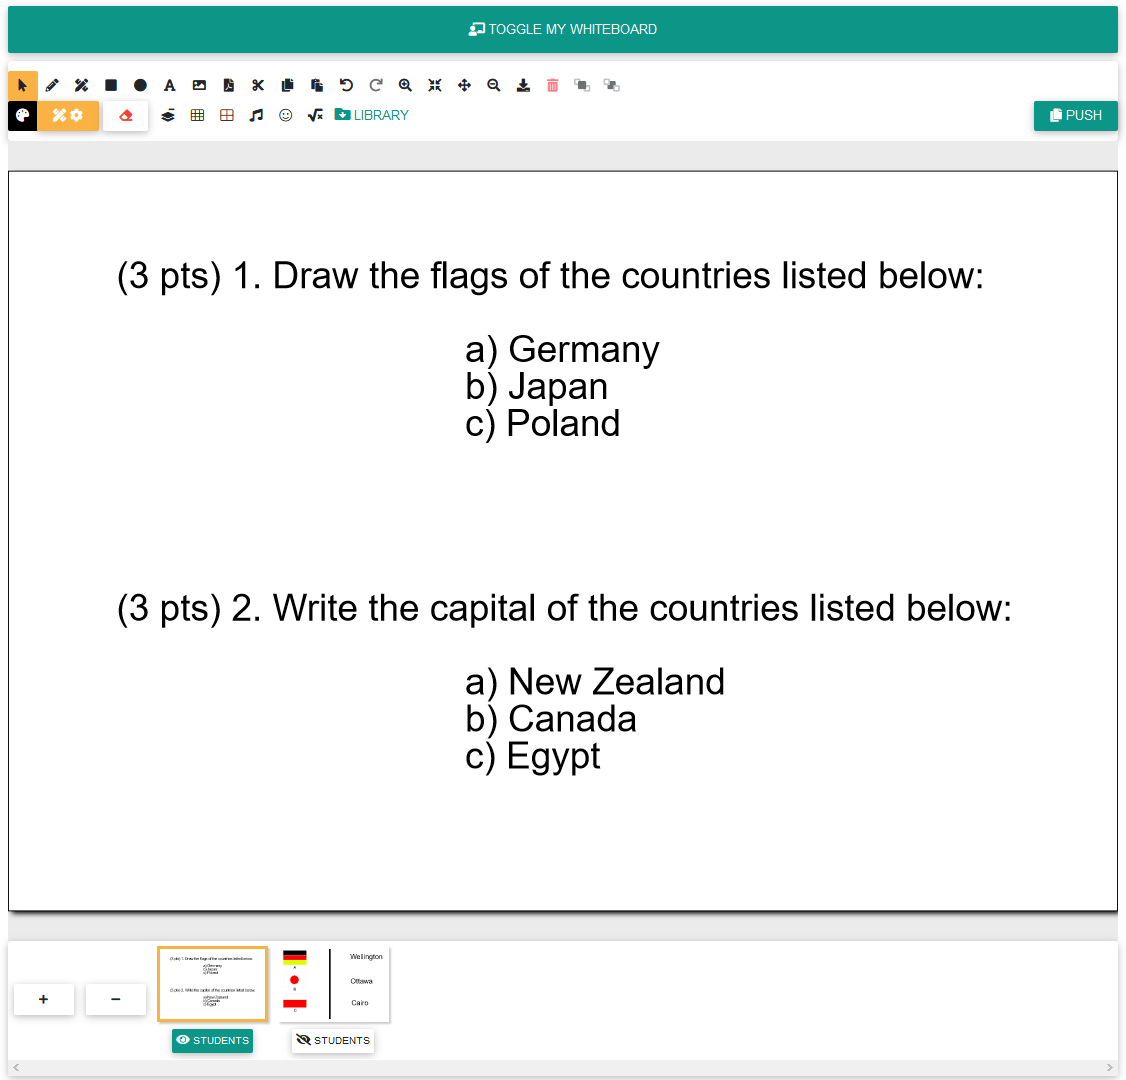
\includegraphics[height=0.7\paperheight]{Figures/whiteboard.png}
        \caption{Snímek webu whiteboard.fi}
    \end{figure}
\end{frame}

\subsection{Analýza stávajících řešení -- miro.com}
\begin{frame}
    \frametitle{Analýza stávajících řešení -- miro.com}
    \begin{figure}
        \centering
        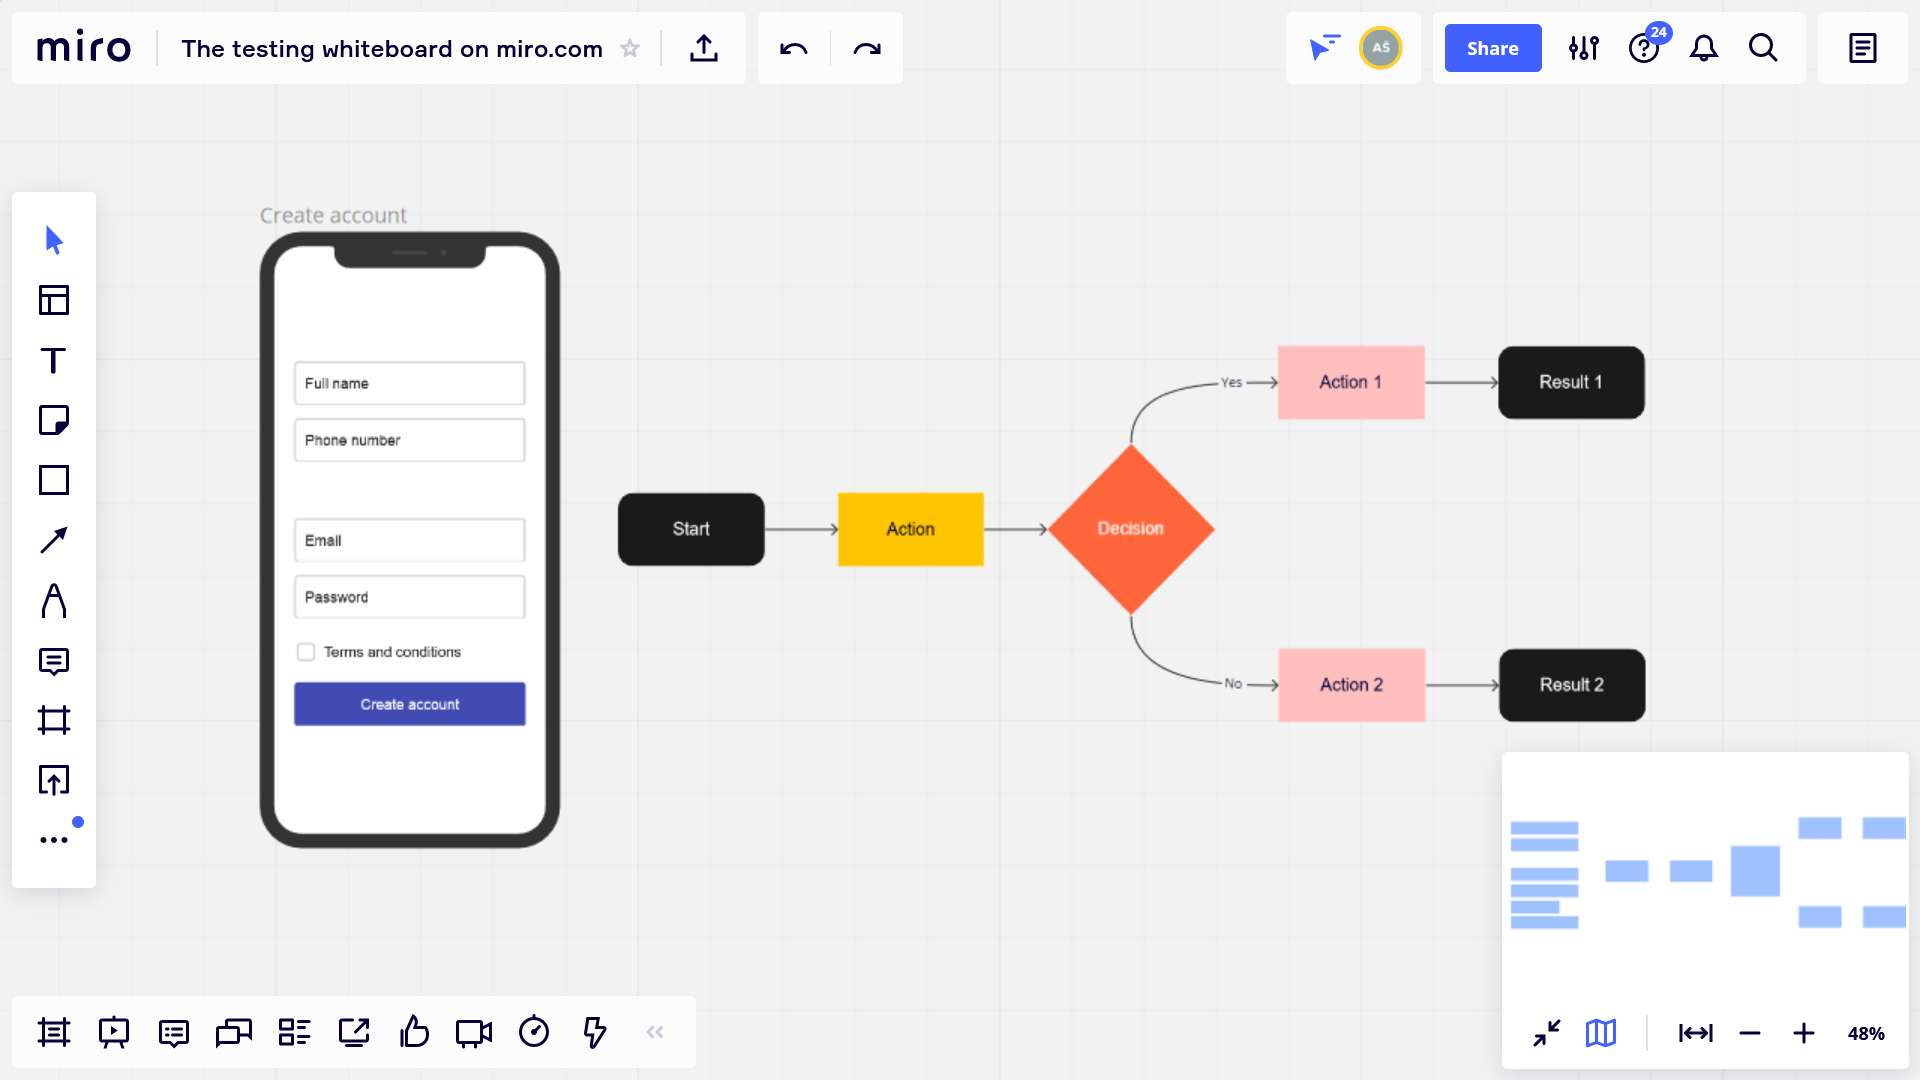
\includegraphics[width=1\textwidth]{Figures/miro.png}
        \caption{Snímek webu miro.com}
    \end{figure}
\end{frame}



\section{Implementace}
\subsection{Vykreslování obsahu}
\subsubsection{Vykreslování obsahu -- problémy}
\begin{frame}
    \frametitle{Vykreslování obsahu -- problémy}
    \begin{itemize}
        \item Tabule se seká či nereaguje vůbec
        \item Objekty se objevují jinde než by měly
        \item Tmavé objekty nejsou na tmavém motivu vidět
    \end{itemize}
\end{frame}

\subsubsection{Vykreslování obsahu -- řešení}
\begin{frame}
    \frametitle{Vykreslování obsahu -- řešení}
    \begin{itemize}
        \item Vytvoření více Canvas elementů
        \item Optimalizace vykreslovacího cyklu
        \item Využití vláken (Web workers)
        \bigskip
        \item Zavedení jednotného systému souřadnic
        \bigskip
        \item Změna jasu barvy dle vybraného motivu
    \end{itemize}
\end{frame}

\subsubsection{Vykreslování obsahu -- ukázky}
\begin{frame}
    \frametitle{Vykreslování obsahu -- ukázka 1}
    \begin{figure}
        \centering
        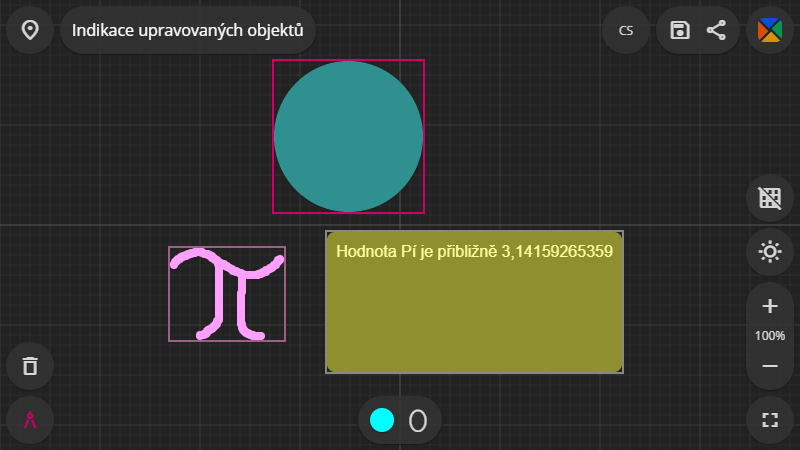
\includegraphics[width=1\textwidth]{Figures/ObjectIndication2.png}
        \caption{Ukázka řešení (tmavý motiv)}
    \end{figure}
\end{frame}

\begin{frame}
    \frametitle{Vykreslování obsahu -- ukázka 2}
    \begin{figure}
        \centering
        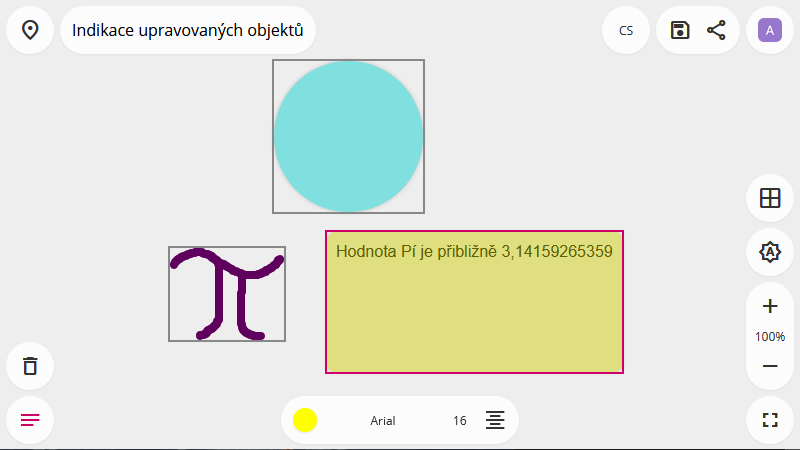
\includegraphics[width=1\textwidth]{Figures/ObjectIndication3.png}
        \caption{Ukázka řešení (světlý motiv)}
    \end{figure}
\end{frame}

\subsection{Propojení se serverem}
\begin{frame}
    \frametitle{Propojení se serverem}
    \begin{figure}
        \centering
        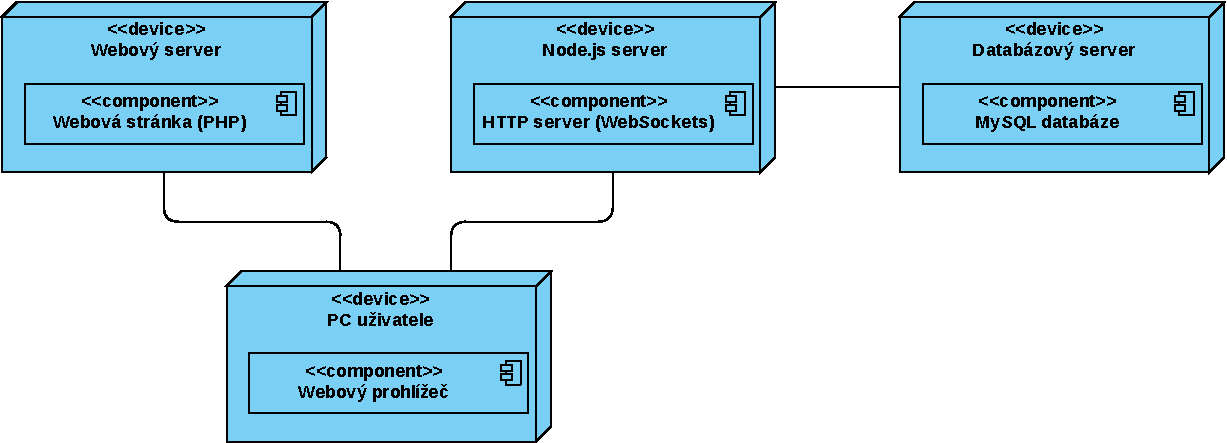
\includegraphics[width=1\textwidth]{Figures/DeploymentDiagram.pdf}
        \caption{Diagram nasazení systému}
    \end{figure}
\end{frame}

\subsubsection{WebSocket server}
\begin{frame}
    \frametitle{WebSocket server}
    \begin{itemize}
        \item Rozesílá data dalším uživatelům tabule
        \item Přenáší data z a do databáze
    \end{itemize}
\end{frame}

\subsection{Jak s daty dále pracovat?}
\begin{frame}
    \frametitle{Jak s daty dále pracovat?}
    \begin{itemize}
        \item Uložení dat do MySQL databáze
        \item Uložení uživatelských výběrů do LocalStorage
        \item Exportování tabule
        \begin{itemize}
            \item Rastrový obrázek
            \item Zdrojový soubor (.json)
        \end{itemize}
    \end{itemize}
\end{frame}

\subsubsection{Relační model databáze}
\begin{frame}
    \frametitle{Relační model databáze}
    \begin{figure}
        \centering
        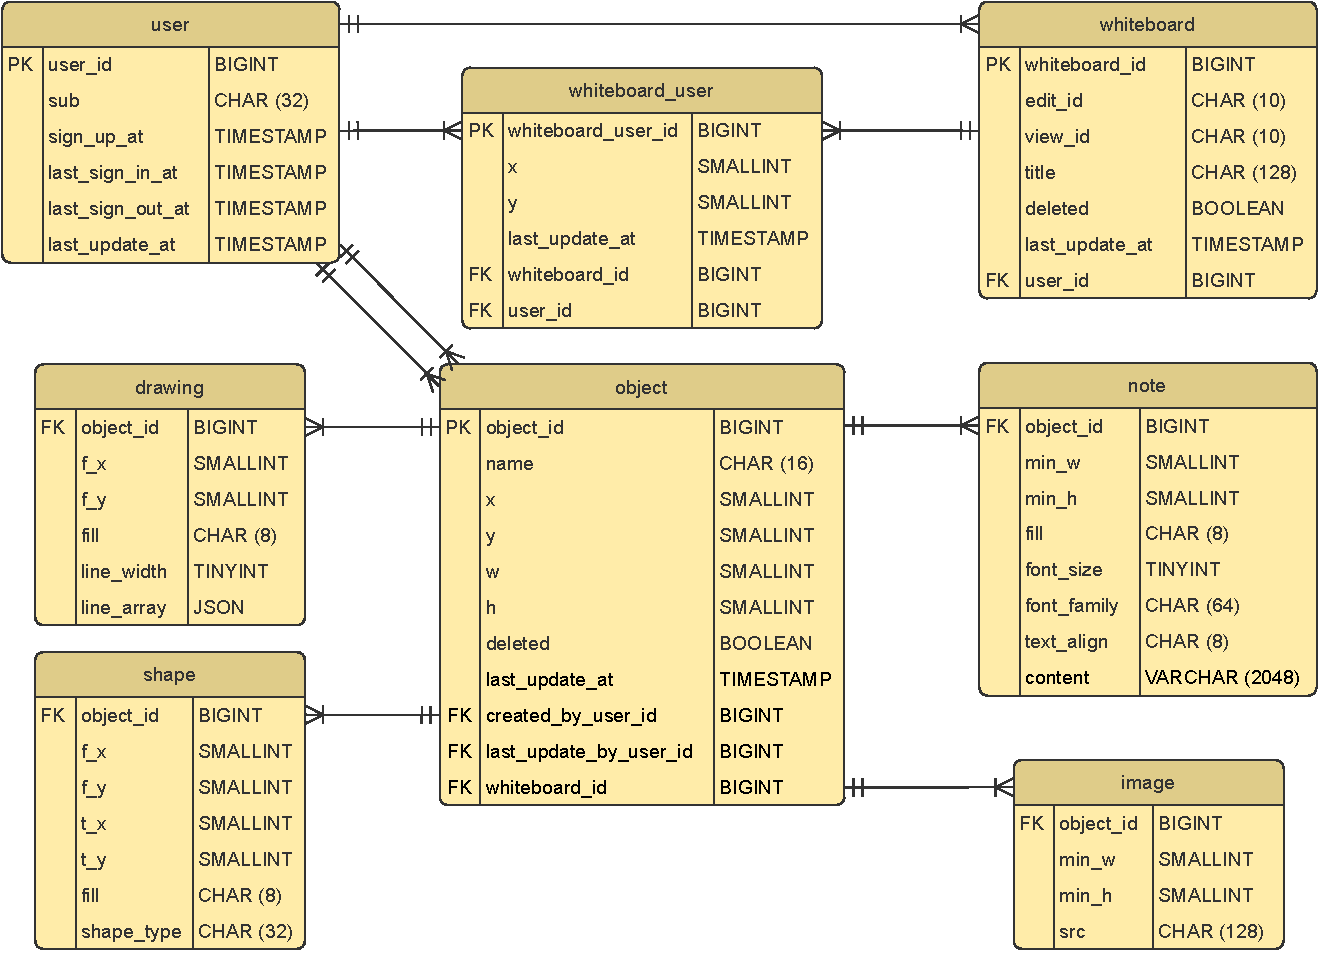
\includegraphics[width=0.8\textwidth]{Figures/EntityRelationshipDiagram.pdf}
        \caption{Relační model databáze}
    \end{figure}
\end{frame}

\subsection{Uživatelské rozhraní}
\begin{frame}
    \frametitle{Uživatelské rozhraní}
    \begin{columns}[T]
        \begin{column}{.67\textwidth}
            \begin{itemize}
                \item Přehledné a intuitivní
                \item Dynamické -- reagující na provedené změny
                \item Responzivní -- použitelné na více typech zařízení
            \end{itemize}
        \end{column}
        \begin{column}{.33\textwidth}
            \begin{figure}
                \centering
    	           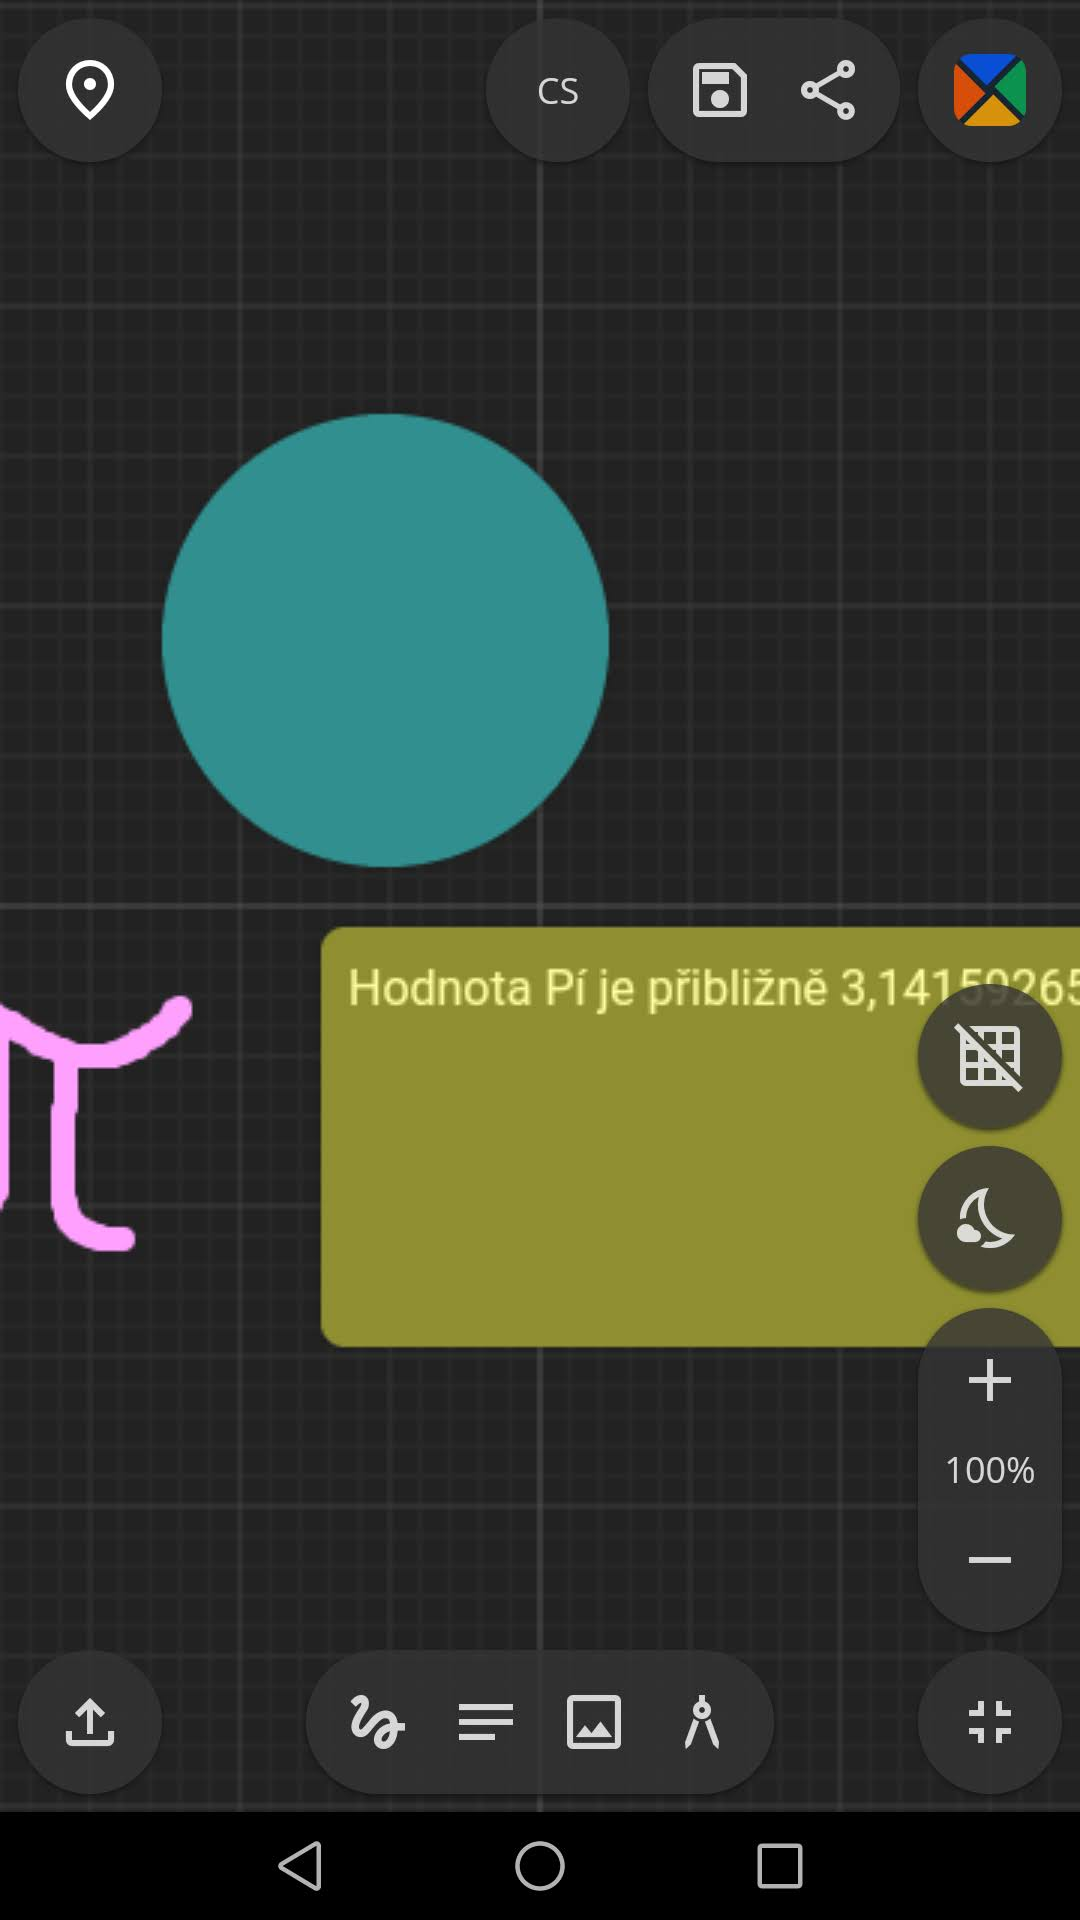
\includegraphics[width=1\textwidth]{Figures/PhoneVersion.jpg}
    	           \caption{Mobilní verze}
            \end{figure}
        \end{column}
    \end{columns}
\end{frame}



\section{Závěr}
\begin{frame}
    \frametitle{Závěr}
\center Děkuji za pozornost.
\end{frame}



\section{Zdroje}
\begin{frame}
    \frametitle{Zdroje}
    {\large\textbf{Seznam použitých obrázků}}
    \begin{itemize}
        \item Snímek webu classroomscreen.com
        \newline
        \noindent https://classroomscreen.com/
        \item Snímek webu whiteboard.fi
        \newline
        \noindent https://whiteboard.fi/
        \item Snímek webu miro.com
        \newline
        \noindent https://miro.com/
    \end{itemize}
\end{frame}
\end{document}
